\begin{figure}[t]
\begin{center}
\begin{subfigure}[t]{0.98\textwidth}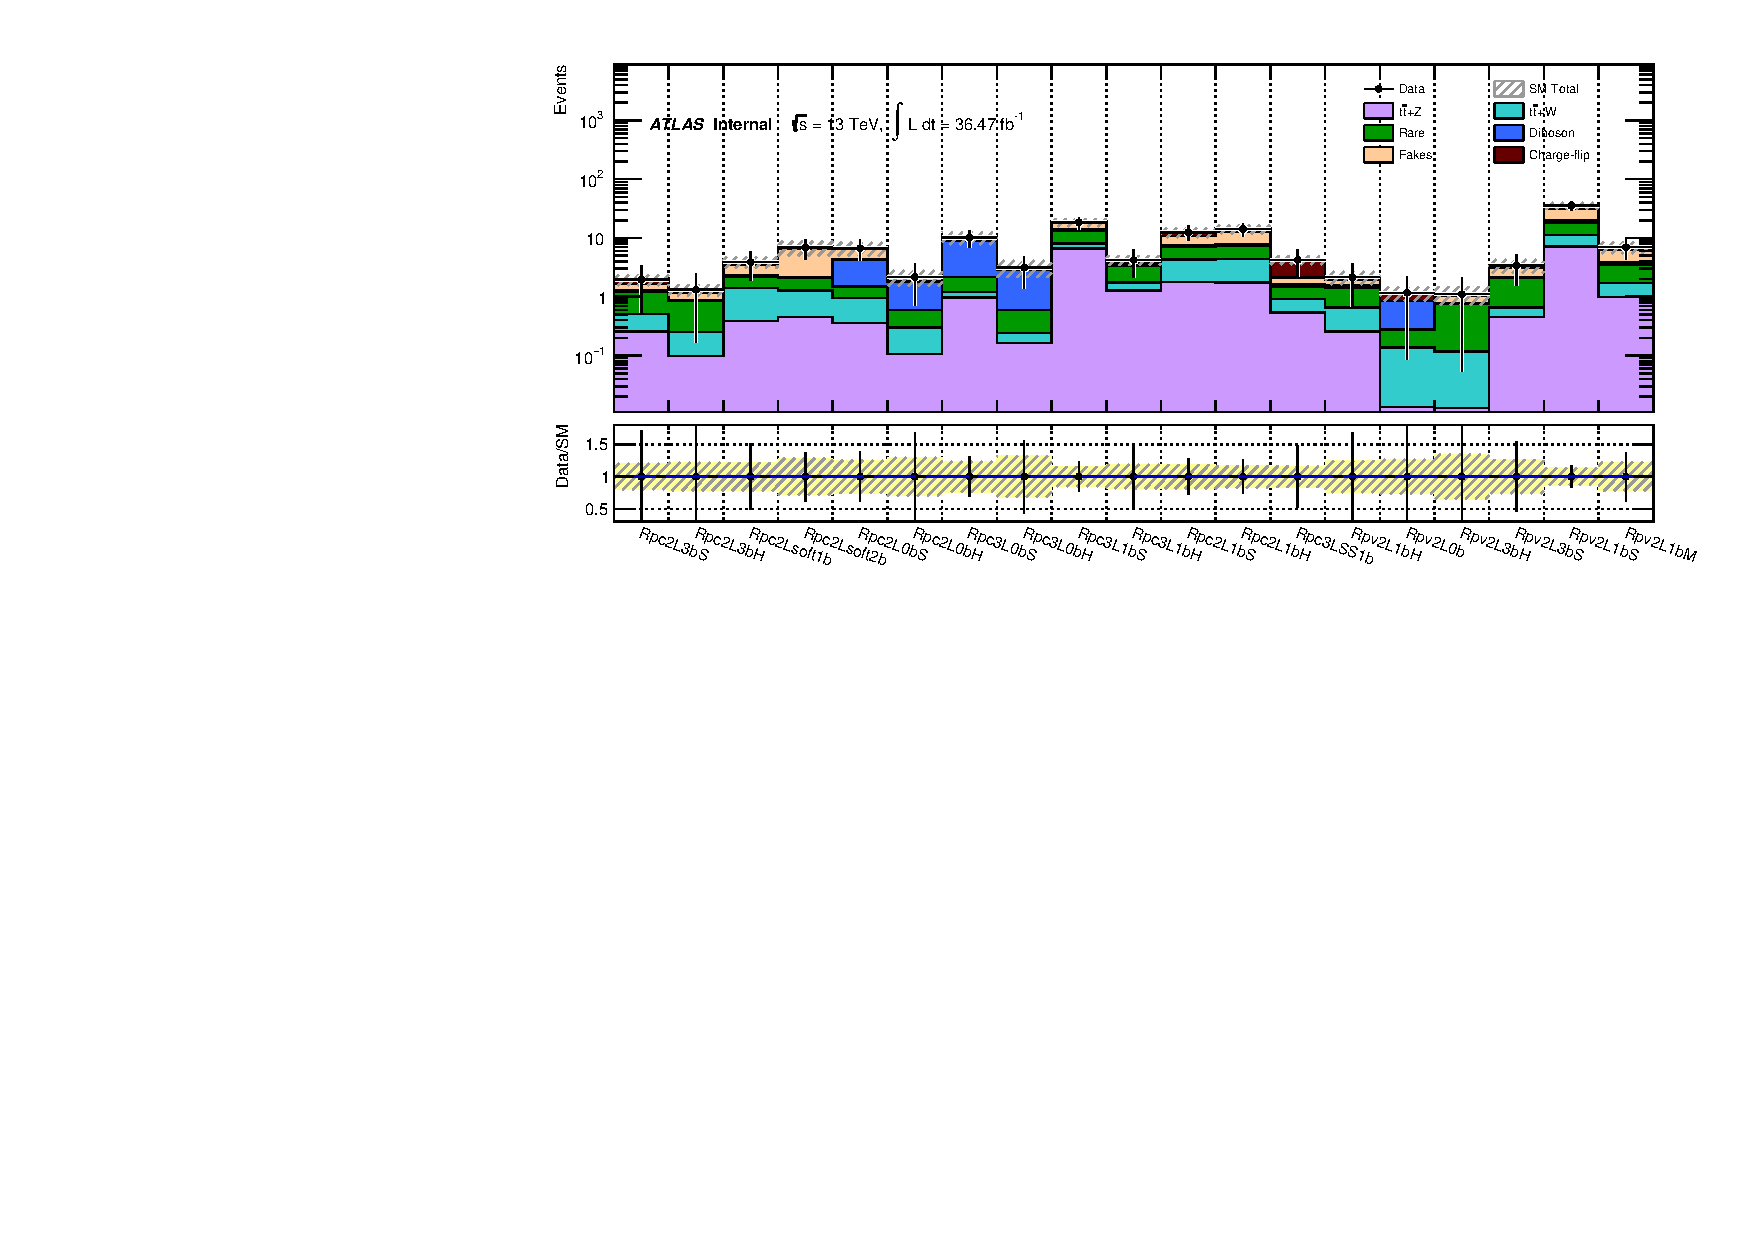
\includegraphics[width=\textwidth]{SRsummary}\caption{}\label{fig:Results_SRSum}\end{subfigure}
\begin{subfigure}[t]{1.08\textwidth}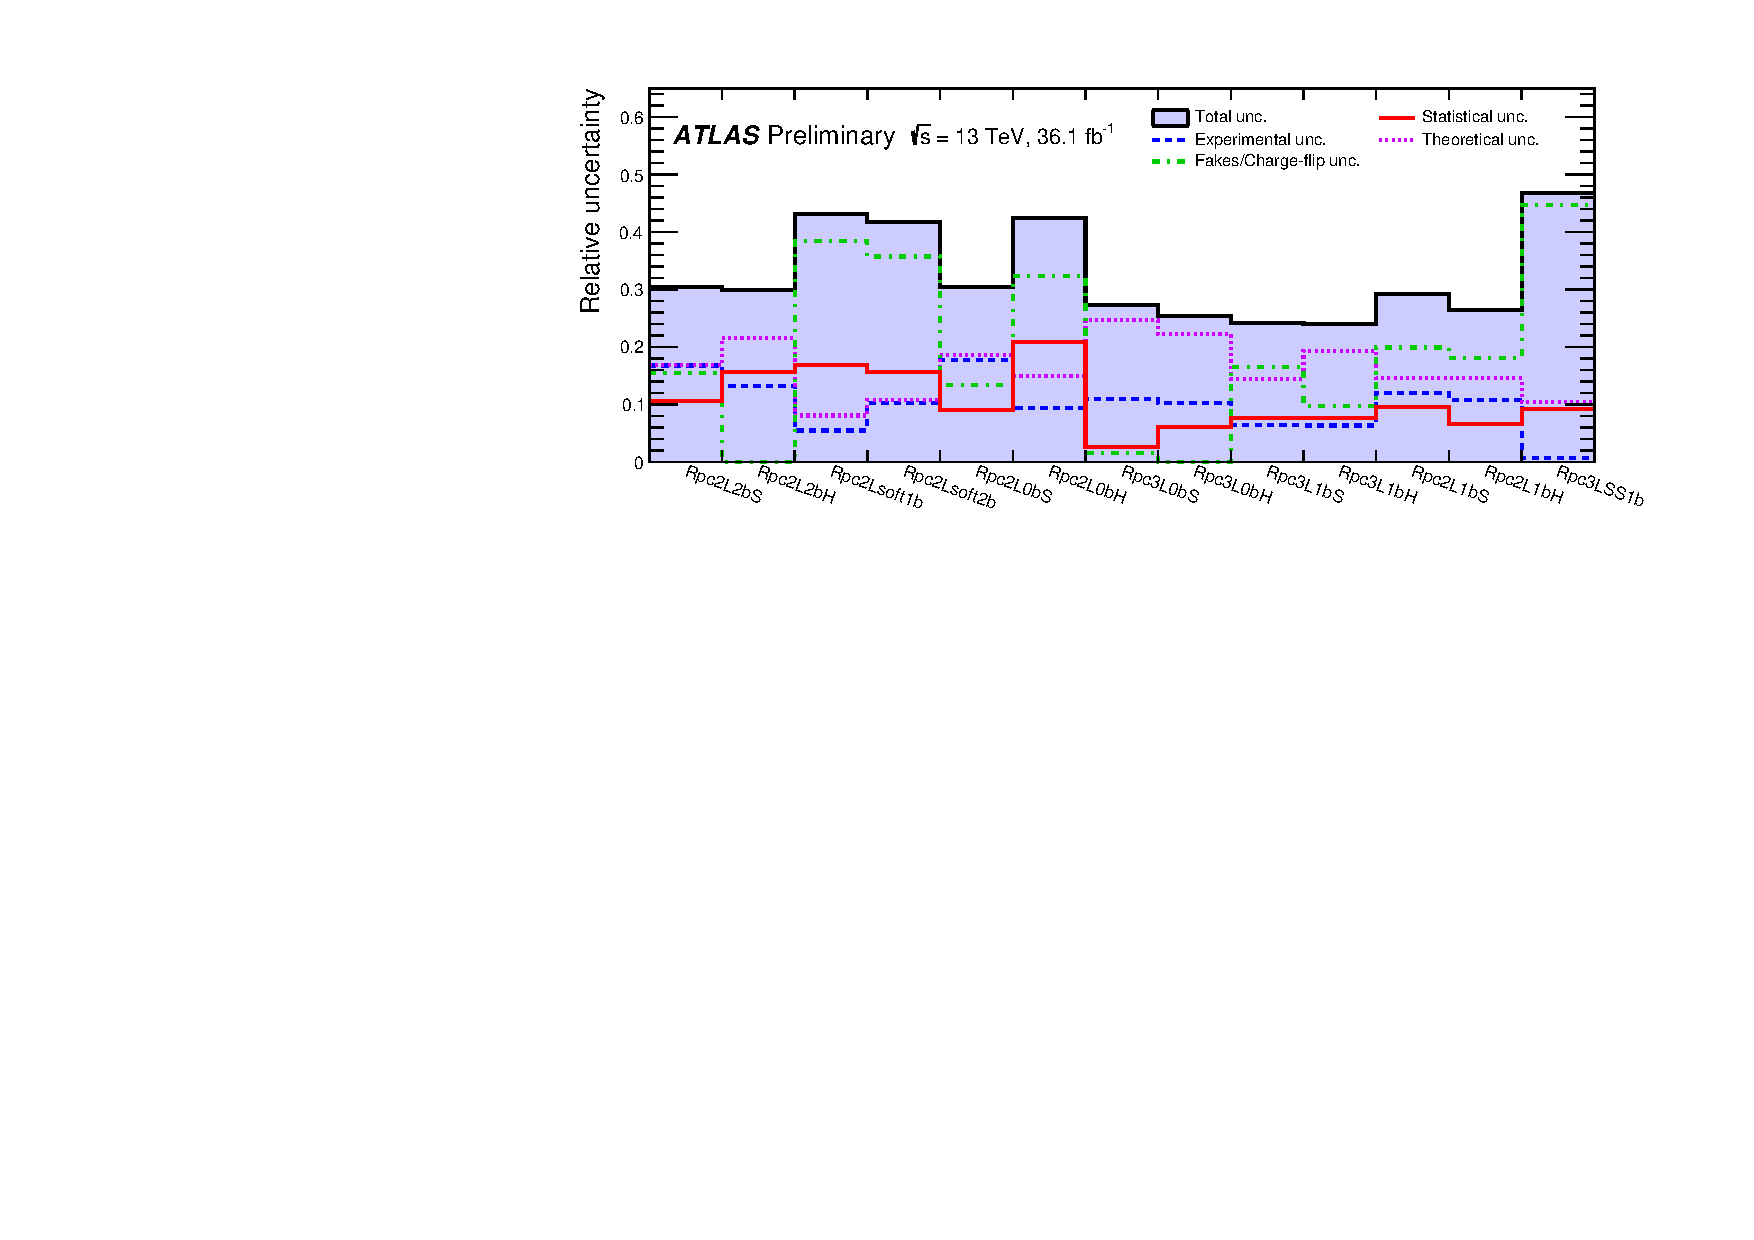
\includegraphics[width=\textwidth]{SystematicsSummary}\caption{}\label{fig:Results_SystSum}\end{subfigure}
\end{center}
\caption{Comparison of (a) the observed and expected event yields in each signal region and (b) the relative uncertainties in the total 
background yield estimate. For the latter, ``statistical uncertainty'' corresponds to reducible and irreducible background 
statistical uncertainties. The background predictions correspond to those presented in Table~\ref{tab:SR_yields} and the 
rare category is explained in the text. } 
\label{fig:PlotSR}
\end{figure}

Figure~\ref{fig:Results_SRSum} shows the event yields for data and the expected background contributions 
in all signal regions. Detailed information about the yields can be found in Table~\ref{tab:SR_yields}.
In all 19 SRs the number of observed data events is consistent with the expected background within the uncertainties. 
The contributions listed in the rare category are dominated by triboson, $tWZ$ and $\ttbar WW$ production.
The triboson processes generally dominate in the SRs with no $b$-jets, while $tWZ$ and $\ttbar WW$
dominate in the SRs with one and two $b$-jets, respectively. Contributions from $WH$, $ZH$, $tZ$ and $\ttbar t$ production 
never represent more than 20\% of the rare background.

\begin{table}
\scriptsize
%\small
\begin{center}
\vspace*{-0.035\textwidth}
\begin{tabular}{|l|c|c|c|c|c|c|}
\hline
Signal Region                  & \textbf{Rpc2L2bS} & \textbf{Rpc2L2bH}    & \textbf{Rpc2Lsoft1b} &\textbf{Rpc2Lsoft2b}& \textbf{Rpc2L0bS} & \textbf{Rpc2L0bH}\\
\hline
\hline
$\ttbar W$, $\ttbar Z\gamma^*$ & $1.6\pm0.4$       & $0.44\pm0.14$     & $1.3\pm0.4$       & $1.21\pm0.33$       & $0.82\pm0.31$       & $0.20\pm0.10$  \\
$\ttbar H$                     & $0.43\pm0.25$     & $0.10\pm0.06$     & $0.45\pm0.24$     & $0.36\pm0.21$       & $0.27\pm0.15$       & $0.08\pm0.07$   \\
4$t$                           & $0.26\pm0.13$     & $0.18\pm0.09$     & $0.09\pm0.05$     & $0.21\pm0.11$       & $0.01\pm0.01$       & $0.02\pm0.02$   \\
Diboson                        & $0.10\pm0.10$     & $0.04\pm0.02$     & $0.17\pm0.09$     & $0.05\pm0.03$       & $3.1\pm1.4$         & $1.0\pm0.5$   \\
Rare                           & $0.33\pm0.18$     & $0.15\pm0.09$     & $0.18\pm0.10$     & $0.17\pm0.10$       & $0.19\pm0.11$       & $0.17\pm0.10$   \\
Fake/non-prompt leptons        & $0.5\pm0.6$       & $0.15\pm0.15$     & $3.5\pm2.4$       & $1.7\pm1.5$         & $1.6\pm1.0$         & $0.9\pm0.9$   \\
Charge-flip                    & $0.10\pm0.01$     & $0.02\pm0.01$     & $0.08\pm0.02$     & $0.08\pm0.02$       & $0.05\pm0.01$       & $0.01\pm0.01$   \\ 
\hline
Total Background               & $3.3\pm1.0$       & $1.08\pm0.32$     & $5.8\pm2.5$       & $3.8 \pm1.6$        & $6.0\pm1.8$         & $2.4\pm1.0$   \\
\hline
Observed                       & $3$               & $0$               & $4$               & $5$                 & $7$                 & $3$   \\
\hline\hline
$S_{\textrm{obs}}^{95}$        & \ral{$5.5$}               & \ral{$3.6$}               & \ral{$6.3$}               & \ral{$7.7$}               & \ral{$8.3$}               & \ral{$6.1$}  \\
$S_{\textrm{exp}}^{95}$        & \ral{$5.6_{-1.5}^{+2.2}$} & \ral{$3.9_{-0.4}^{+1.4}$} & \ral{$7.1_{-1.5}^{+2.5}$} & \ral{$6.2_{-1.5}^{+2.6}$} & \ral{$7.5_{-1.8}^{+2.6}$} & \ral{$5.3_{-1.3}^{+2.1}$} \\
$\sigma_{\textrm{vis}}$ [fb]   & \ral{$0.15$}              & \ral{$0.10$}              & \ral{$0.17$}              & \ral{$0.21$}              & \ral{$0.23$}              & \ral{$0.17$}  \\
$p_{0}$ ($\textrm{Z}$)         & \ral{$0.71$ (--)}         & \ral{$0.91$ (--)}         & \ral{$0.69$ (--)}         & \ral{$0.30\ (0.5\sigma)$} & \ral{$0.36\ (0.4\sigma)$} & \ral{$0.35\ (0.4\sigma)$}  \\
\hline 
\end{tabular}

\vspace*{1cm}

\begin{tabular}{|l|c|c|c|c|c|c|c|}
\hline
Signal Region 		& \textbf{Rpc3L0bS } 	& \textbf{Rpc3L0bH } 	& \textbf{Rpc3L1bS } 	& \textbf{Rpc3L1bH } 	& \textbf{Rpc2L1bS } 	& \textbf{Rpc2L1bH } 	& \textbf{Rpc3LSS1b }\\
\hline
\hline
$\ttbar W$, $\ttbar Z\gamma^*$   & $0.98\pm0.25$       	& $0.18\pm0.08$       	& $7.1\pm1.1$       	& $1.54\pm0.28$       	& $4.0\pm1.0$ 		& $4.0\pm0.9$	  	&  --     		\\
$\ttbar H$              & $0.12\pm0.08$       	& $0.03\pm0.02$       	& $1.4\pm0.7$       	& $0.25\pm0.14$       	& $1.3\pm0.7$ 		& $1.0\pm0.6$	  	& $0.22\pm0.12$    	\\
4$t$	   		& $0.02\pm0.01$	  & $0.01\pm0.01$	  & $0.7\pm0.4$ 	  & $0.28\pm0.15$	  & $0.34\pm0.17$	  & $0.54\pm0.28$	  &  -- 		  \\
Diboson                  & $8.9\pm2.9$       	& $2.6\pm0.8$       	& $1.4\pm0.5$       	& $0.48\pm0.17$       	& $0.5\pm0.3$ 		& $0.7\pm0.3$ 		&  --     		\\
Rare                     & $0.7\pm0.4$       	& $0.29\pm0.16$       	& $2.5\pm1.3$       	& $0.9\pm0.5$       	& $0.9\pm0.5$		& $1.0\pm0.6$		& $0.12\pm0.07$    	\\
Fake/non-prompt leptons  & $0.23\pm0.23$       	& $0.15\pm0.15$       	& $4.2\pm3.1$       	& $0.5\pm0.5$       	& $2.5\pm2.2$ 		& $2.3\pm1.9$  		& $0.9\pm0.7$    	\\
Charge-flip              &  --   		&  --    		&  --    		&  --     		& $0.25\pm0.04$ 	& $0.25\pm0.05$  	& $0.39\pm0.08$		\\	
\hline
Total Background         & $11.0\pm3.0\hpO$	       & $3.3\pm0.8$       	& $17\pm4\hpO$       	& $3.9\pm0.9$       	& $9.8\pm2.9$ 		& $9.8\pm2.6$  		& $1.6\pm0.8$	   	\\
\hline
Observed                 & $9$       		& $3$       		& $20$		       	& $4$       		& $14$  		&  $13$    		&  $1$			  \\
\hline\hline
$S_{\textrm{obs}}^{95}$       & \ral{$8.3$}	  	& $5.4$	   		& \ral{$14.7$}	    	& \ral{$6.1$}	     		& \ral{$13.7$}  		& \ral{$12.4$}   		& \ral{$3.9$}     		\\
$S_{\textrm{exp}}^{95}$       & \ral{$9.3_{-2.3}^{+3.1}$}	& \ral{$5.5_{-1.5}^{+2.2}$}	& \ral{$12.6_{-3.4}^{+5.1}$} 	& \ral{$5.9_{-1.8}^{+2.2}$}	& \ral{$10.0_{-2.6}^{+3.7}$}	& \ral{$9.7_{-2.6}^{+3.4}$}   & \ral{$4.0_{-0.3}^{+1.8}$}    \\
$\sigma_{\textrm{vis}}$ [fb] & \ral{$0.23$}		& \ral{$0.15$}  		& \ral{$0.41$}      		& \ral{$0.17$}      		& \ral{$0.38$}  		& \ral{$0.34$}   		& \ral{$0.11$}     		\\
$p_{0}$ ($\textrm{Z}$)        & \ral{$0.72$ (--)}  	& \ral{$0.85$ (--)}  		& \ral{$0.32\ (0.5\sigma)$}  & \ral{$0.46\ (0.1\sigma)$}  	& \ral{$0.17\ (1.0\sigma)$}  	& \ral{$0.21\ (0.8\sigma)$}	& \ral{$0.56$ (--)}	\\
\hline 
\end{tabular}

\vspace*{1cm}


\vspace*{1cm}

\vspace*{-0.01\textheight}\caption{Numbers of events observed in the signal regions compared with the expected backgrounds. 
The rare category is defined in the text. Background categories with yields shown as a ``--'' 
do not contribute to a given region (e.g. charge flips in three-lepton regions) or their estimates are below 0.01. 
The 95\% confidence level (CL) upper limits are shown on the observed and expected numbers of BSM events, $S_{\textrm{obs}}^{95}$ and $S_{\textrm{exp}}^{95}$ 
(as well as the $\pm 1\sigma$ excursions from the expected limit), respectively. The 95\% CL upper limits on the visible cross-section 
($\sigma_{\textrm{vis}}$) are also given. Finally the $p$-values ($p_{0}$) give the probabilities of the observations being consistent 
with the estimated backgrounds. The number of equivalent Gaussian standard deviations ($Z$) is also shown when $p_{0}<0.5$.}
\label{tab:SR_yields}
\end{center}
\end{table}

Figure~\ref{fig:Results_SystSum} summarizes the contributions from the different sources of systematic uncertainty 
to the total SM background predictions in the signal regions. The uncertainties amount to 25--45\% of the 
total background depending on the signal region, dominated by systematic uncertainties coming from the reducible background or the theory. 

In the absence of any significant deviation from the SM predictions, upper limits on possible BSM contributions to the signal regions are derived, 
as well as exclusion limits on the masses of SUSY particles in the benchmark scenarios of Figure~\ref{fig:feynman}. 
The HistFitter framework~\cite{Baak:2014wma}, which utilizes a profile-likelihood-ratio test~\cite{Cowan:2010js}, 
is used to establish 95\% confidence intervals using the CL$_\mathrm{s}$ prescription~\cite{Read:2002hq}. 
The likelihood is built as the product of a Poisson probability density function describing the observed number of events in the signal region 
and, to constrain the nuisance parameters associated with the systematic uncertainties, 
Gaussian distributions whose widths correspond to the sizes of these uncertainties; 
Poisson distributions are used instead for MC simulation statistical uncertainties.
Correlations of a given nuisance parameter between the backgrounds and the signal are taken into account when relevant. 
The hypothesis tests are performed for each of the signal regions independently. 

Table~\ref{tab:SR_yields} presents 95\% confidence level (CL) observed (expected) model-independent upper limits 
on the number of BSM events, $S_{\textrm{obs}}^{95}$ ($S_{\textrm{exp}}^{95}$), that may contribute to the signal regions. 
Normalizing these by the integrated luminosity $L$ of the data sample, they can be interpreted as upper limits on the visible 
BSM cross-section ($\sigma_{\textrm{vis}}$), defined as $\sigma_{\textrm{vis}}=\sigma_{\textrm{prod}}\times A \times\epsilon=S_{\textrm{obs}}^{95}/L$, where 
$\sigma_{\textrm{prod}}$ is the production cross-section, $A$ the acceptance and $\epsilon$ the reconstruction efficiency. The largest 
deviation of the data from the background prediction corresponds to an excess of XX standard deviations in the YY SR.

\begin{figure}[p]
\centering
%\begin{subfigure}[t]{0.38\textwidth}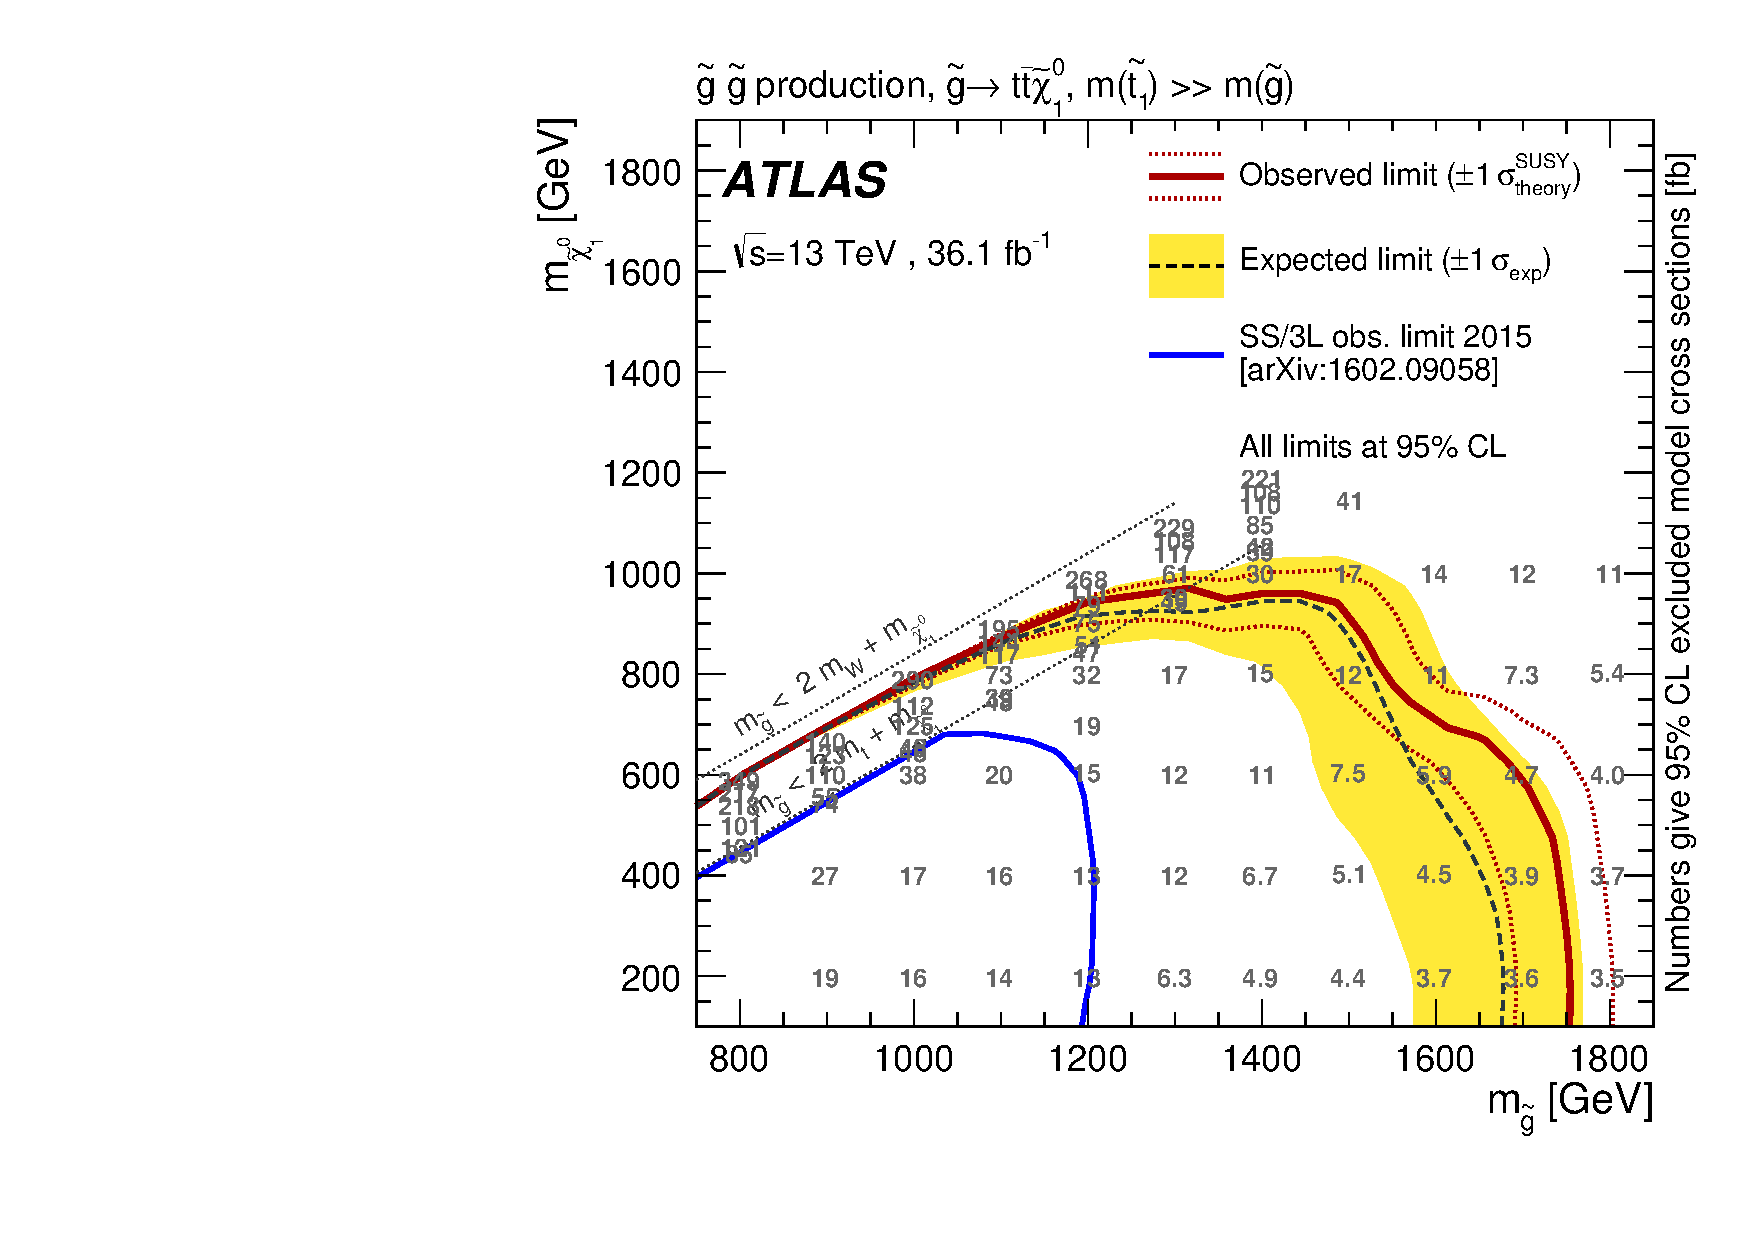
\includegraphics[width=\textwidth]{LIMITS/Gtt_SRbest}\caption{Rpc2L2bS, Rpc2L2bH}\label{fig:limits_feynman_gtt}\end{subfigure}
%\begin{subfigure}[t]{0.38\textwidth}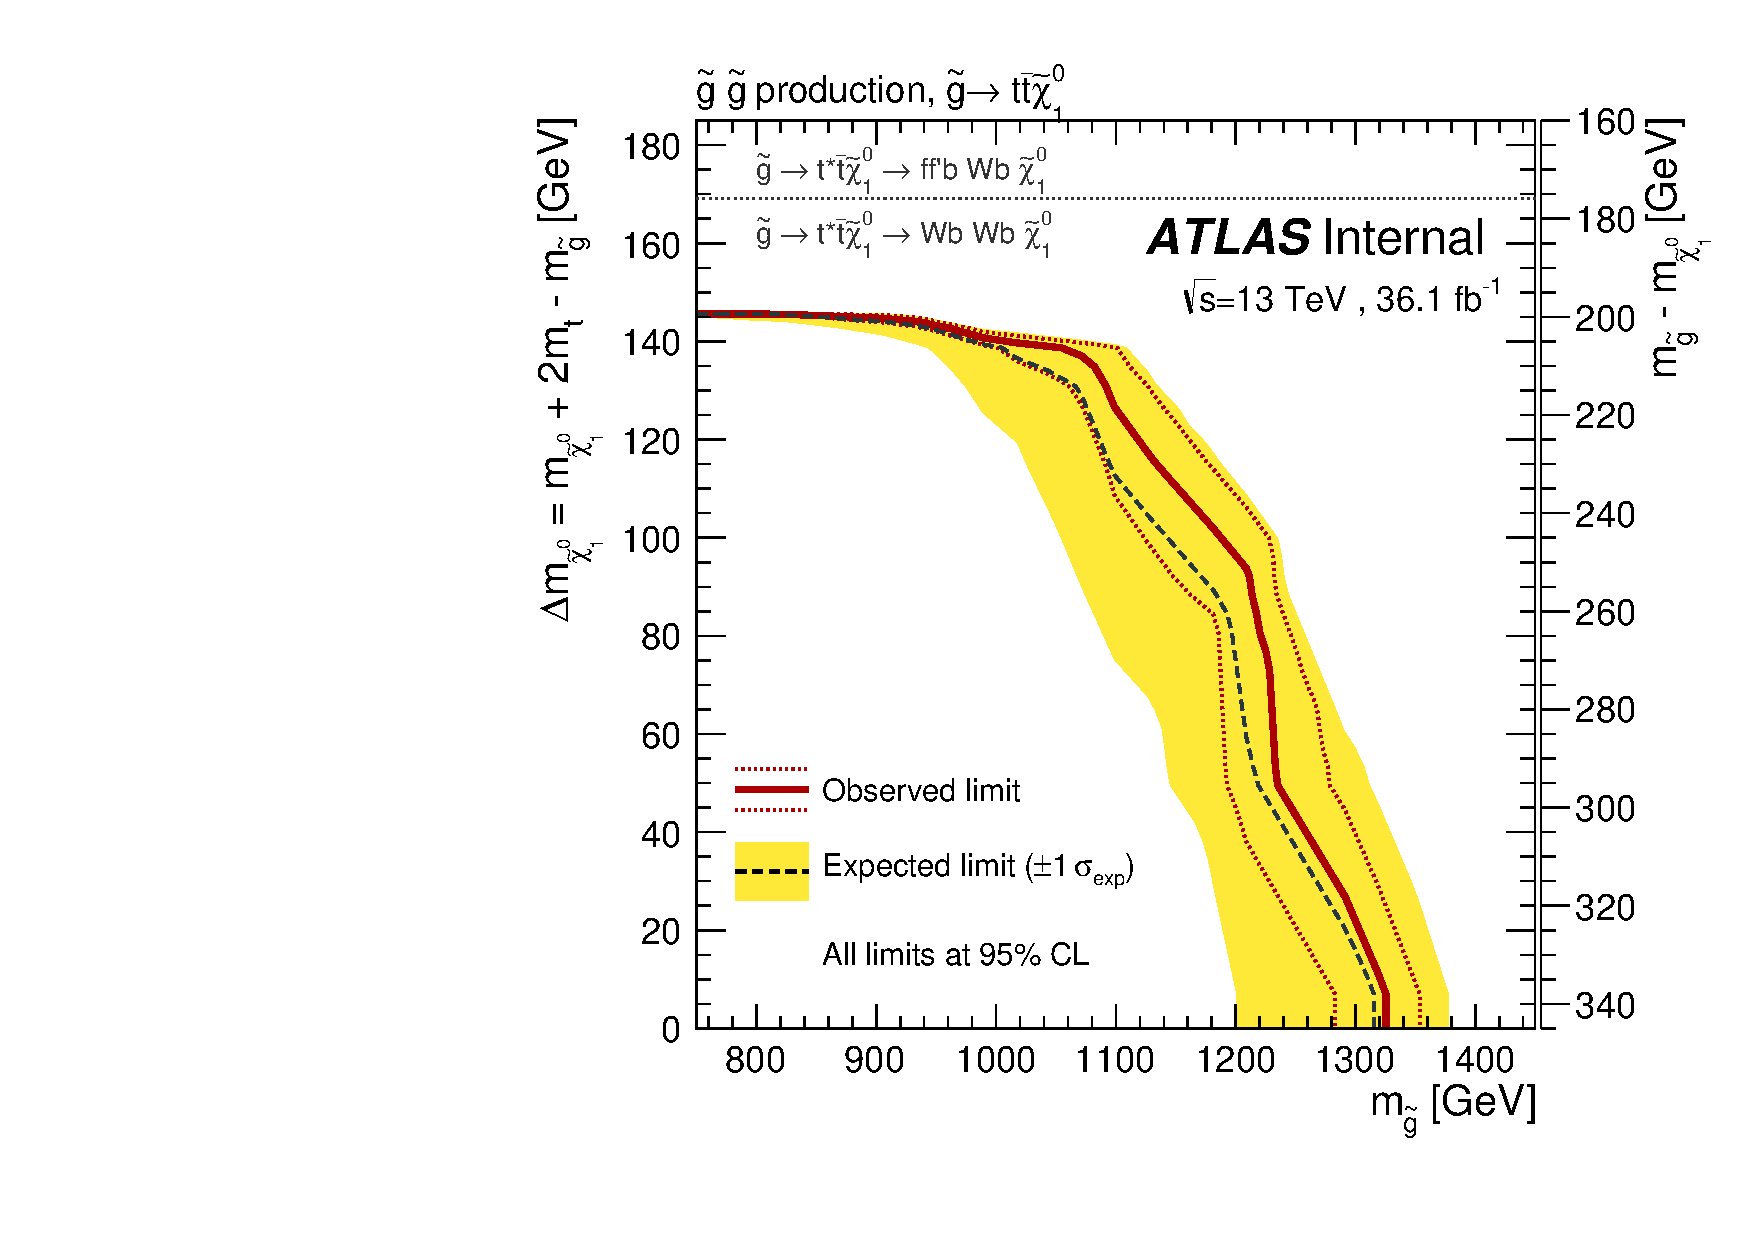
\includegraphics[width=\textwidth]{LIMITS/Gtt_above}\caption{Rpc2Lsoft1b, Rpc2Lsoft2b}\label{fig:limits_feynman_gttOffshell}\end{subfigure}
\begin{subfigure}[t]{0.38\textwidth}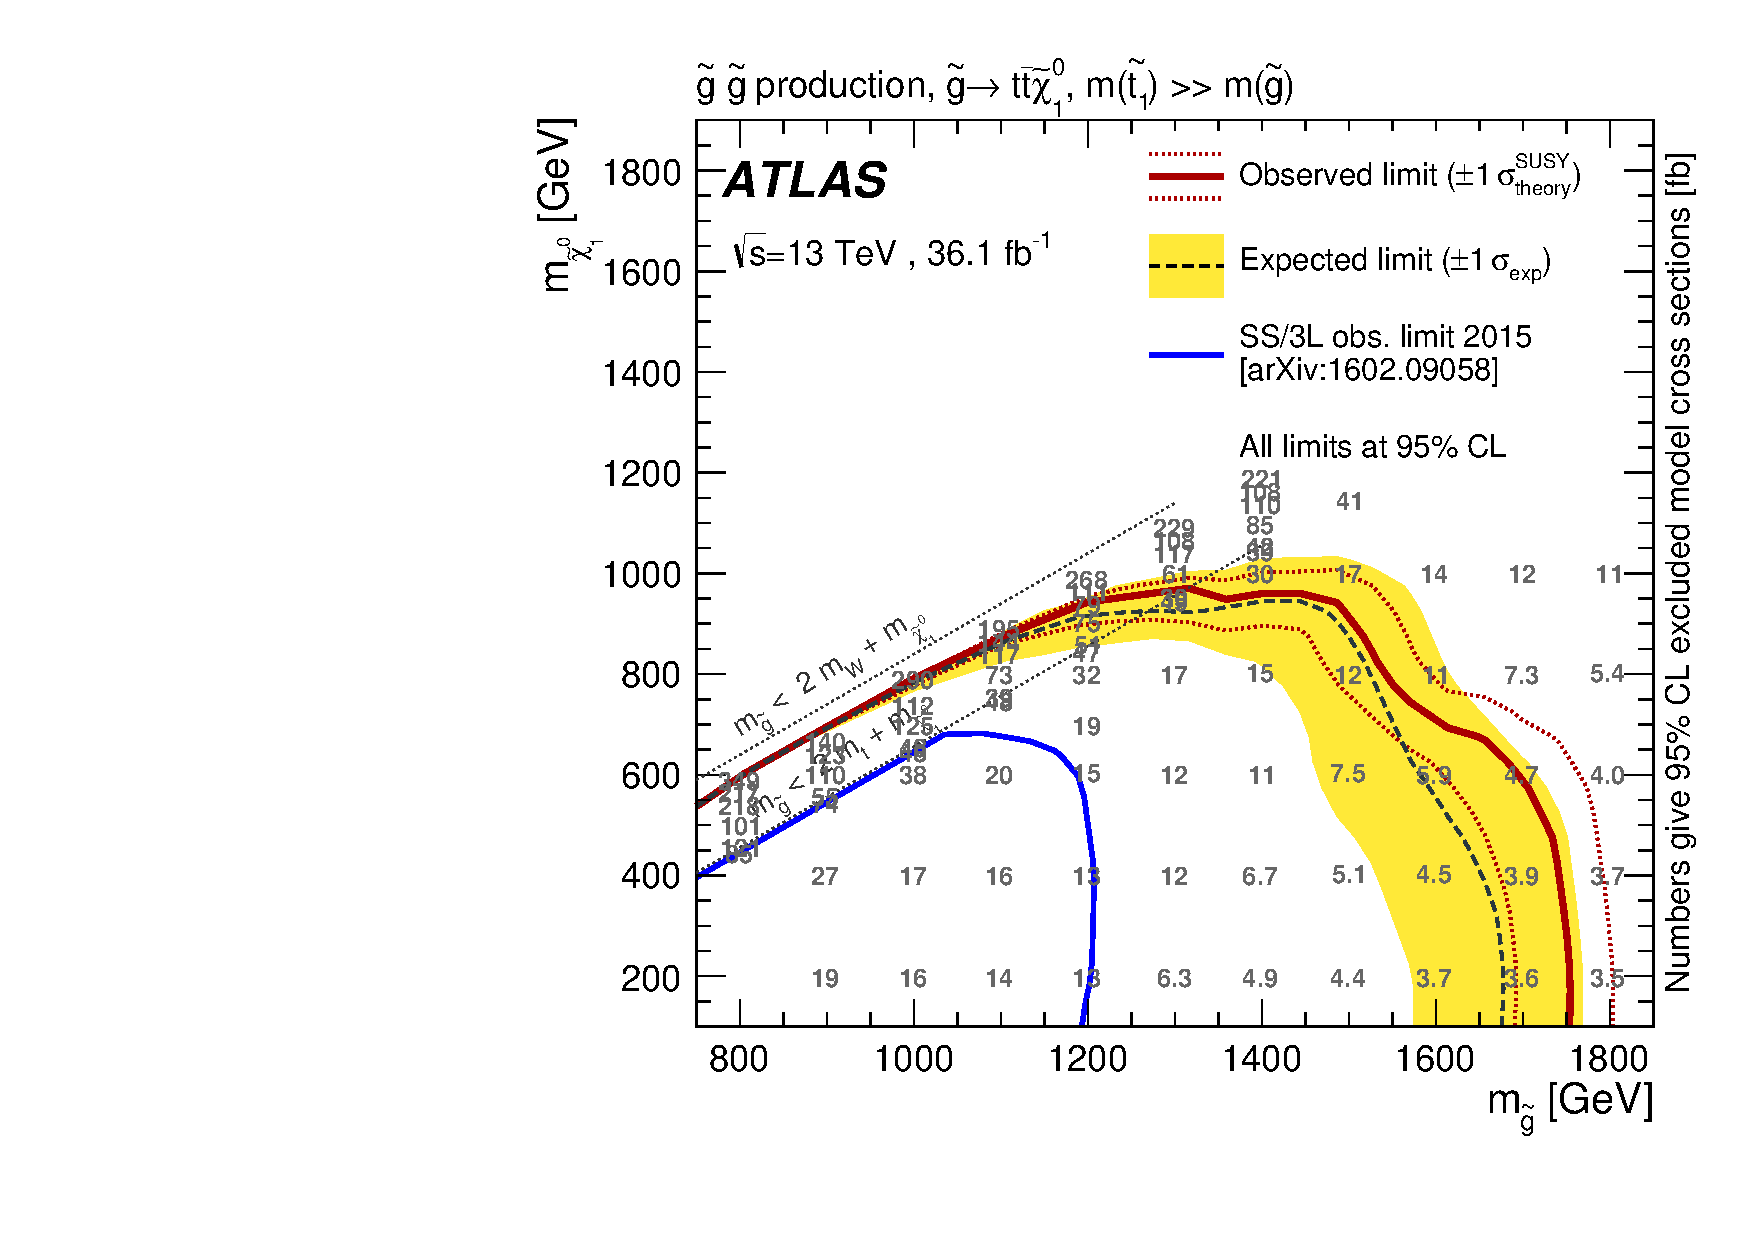
\includegraphics[width=\textwidth]{LIMITS/Gtt_SRbest}\caption{Rpc2L2bS/H, Rpc2Lsoft1b/2b}\label{fig:limits_feynman_gtt}\end{subfigure}
\begin{subfigure}[t]{0.38\textwidth}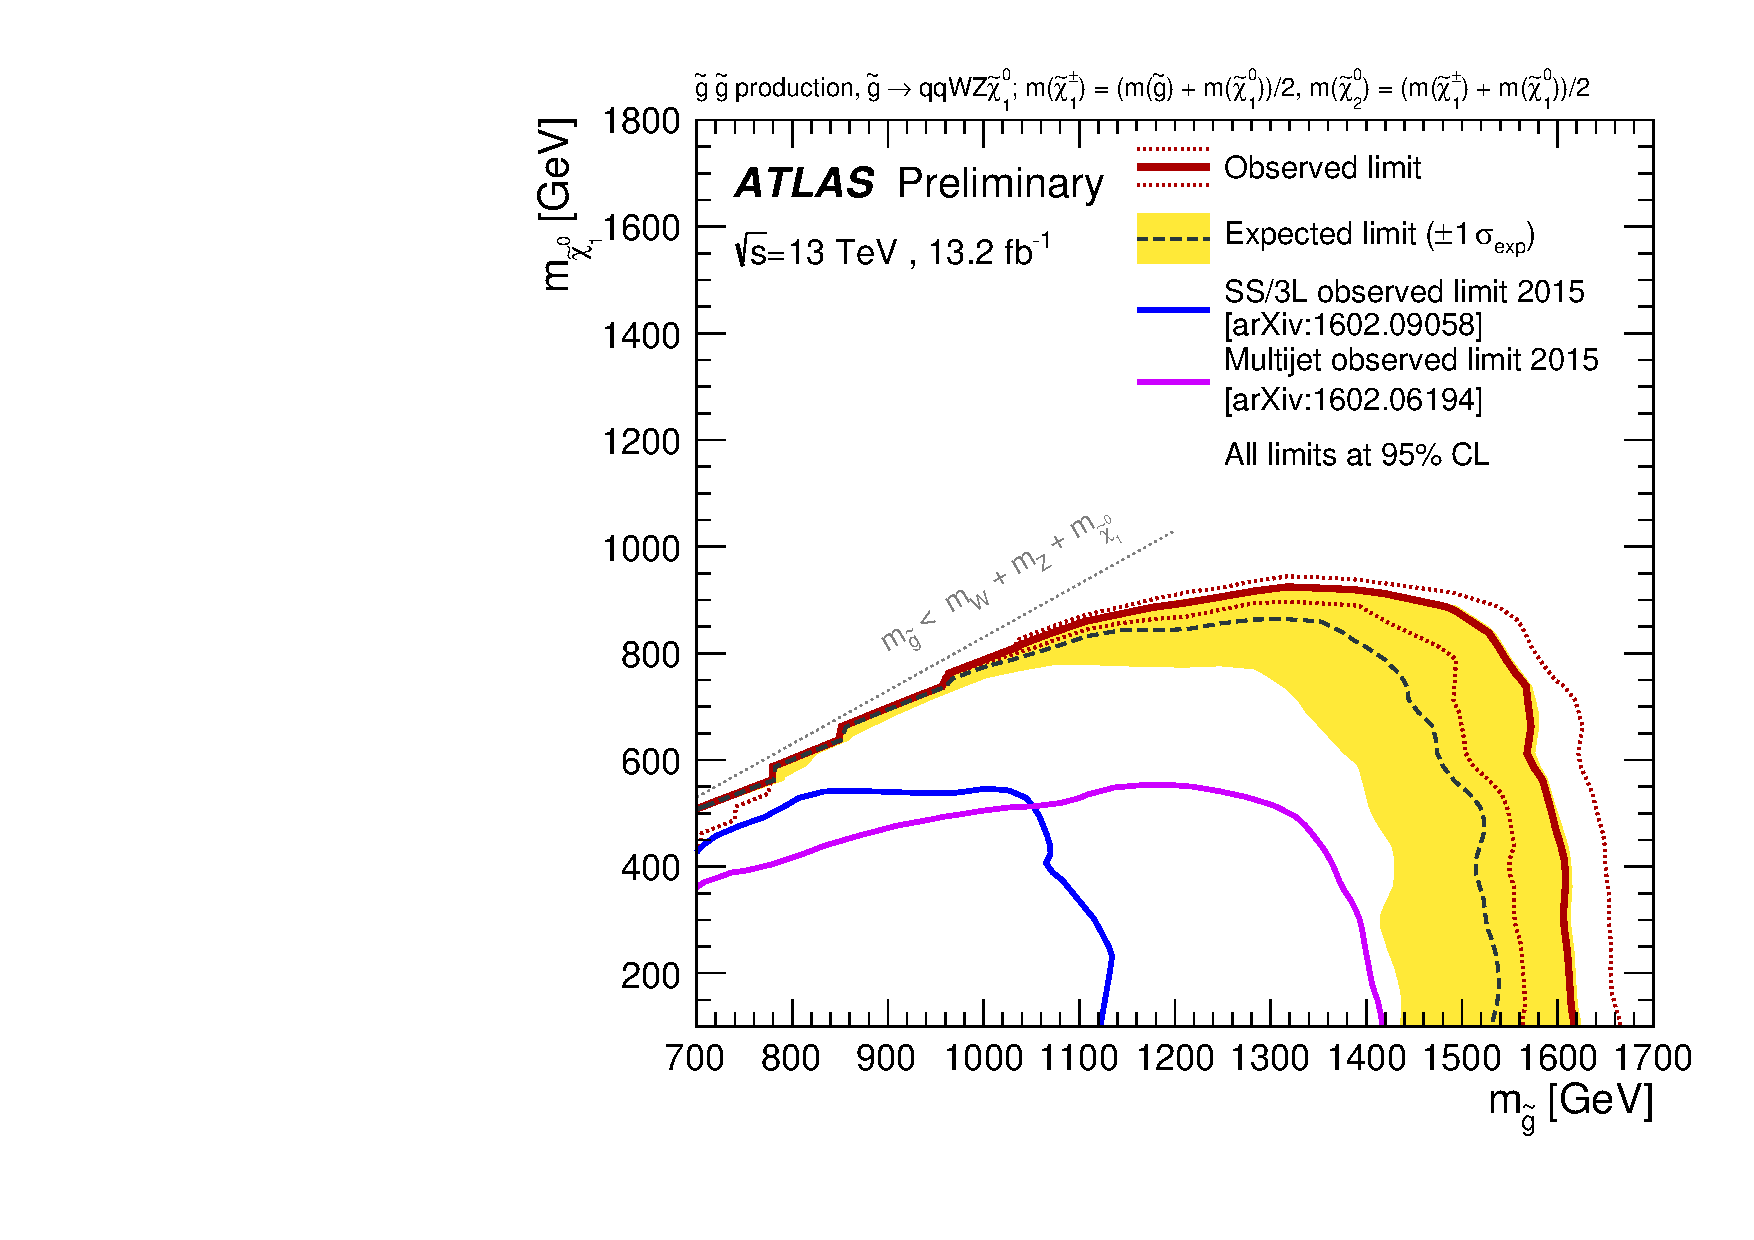
\includegraphics[width=\textwidth]{LIMITS/2stepWZ_SRbest}\caption{Rpc2L0bS, Rpc2L0bH}\label{fig:limits_feynman_gg2WZ}\end{subfigure}
\begin{subfigure}[t]{0.38\textwidth}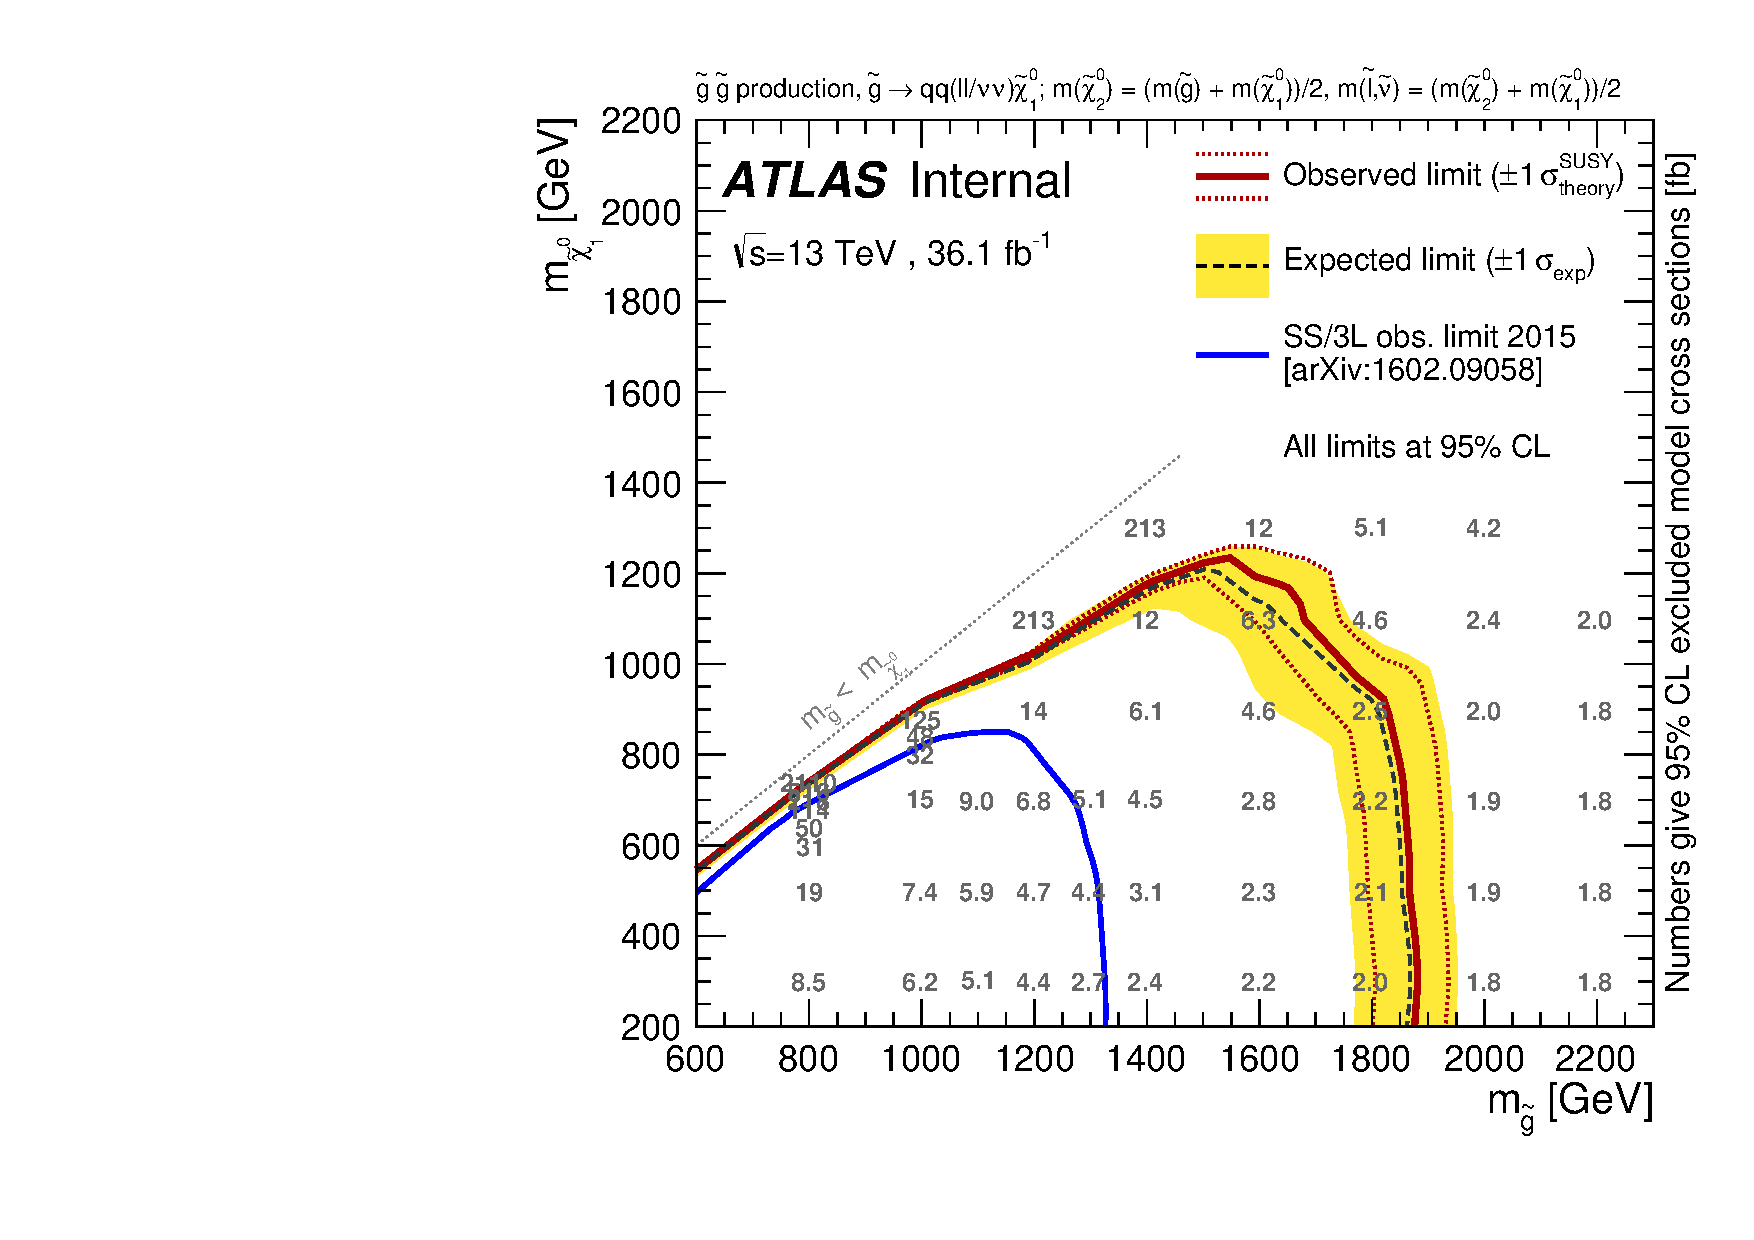
\includegraphics[width=\textwidth]{LIMITS/GSL_SRbest.pdf}\caption{Rpc3L0bS, Rpc3L0bH}\label{fig:limits_feynman_gg2sl}\end{subfigure}
\begin{subfigure}[t]{0.38\textwidth}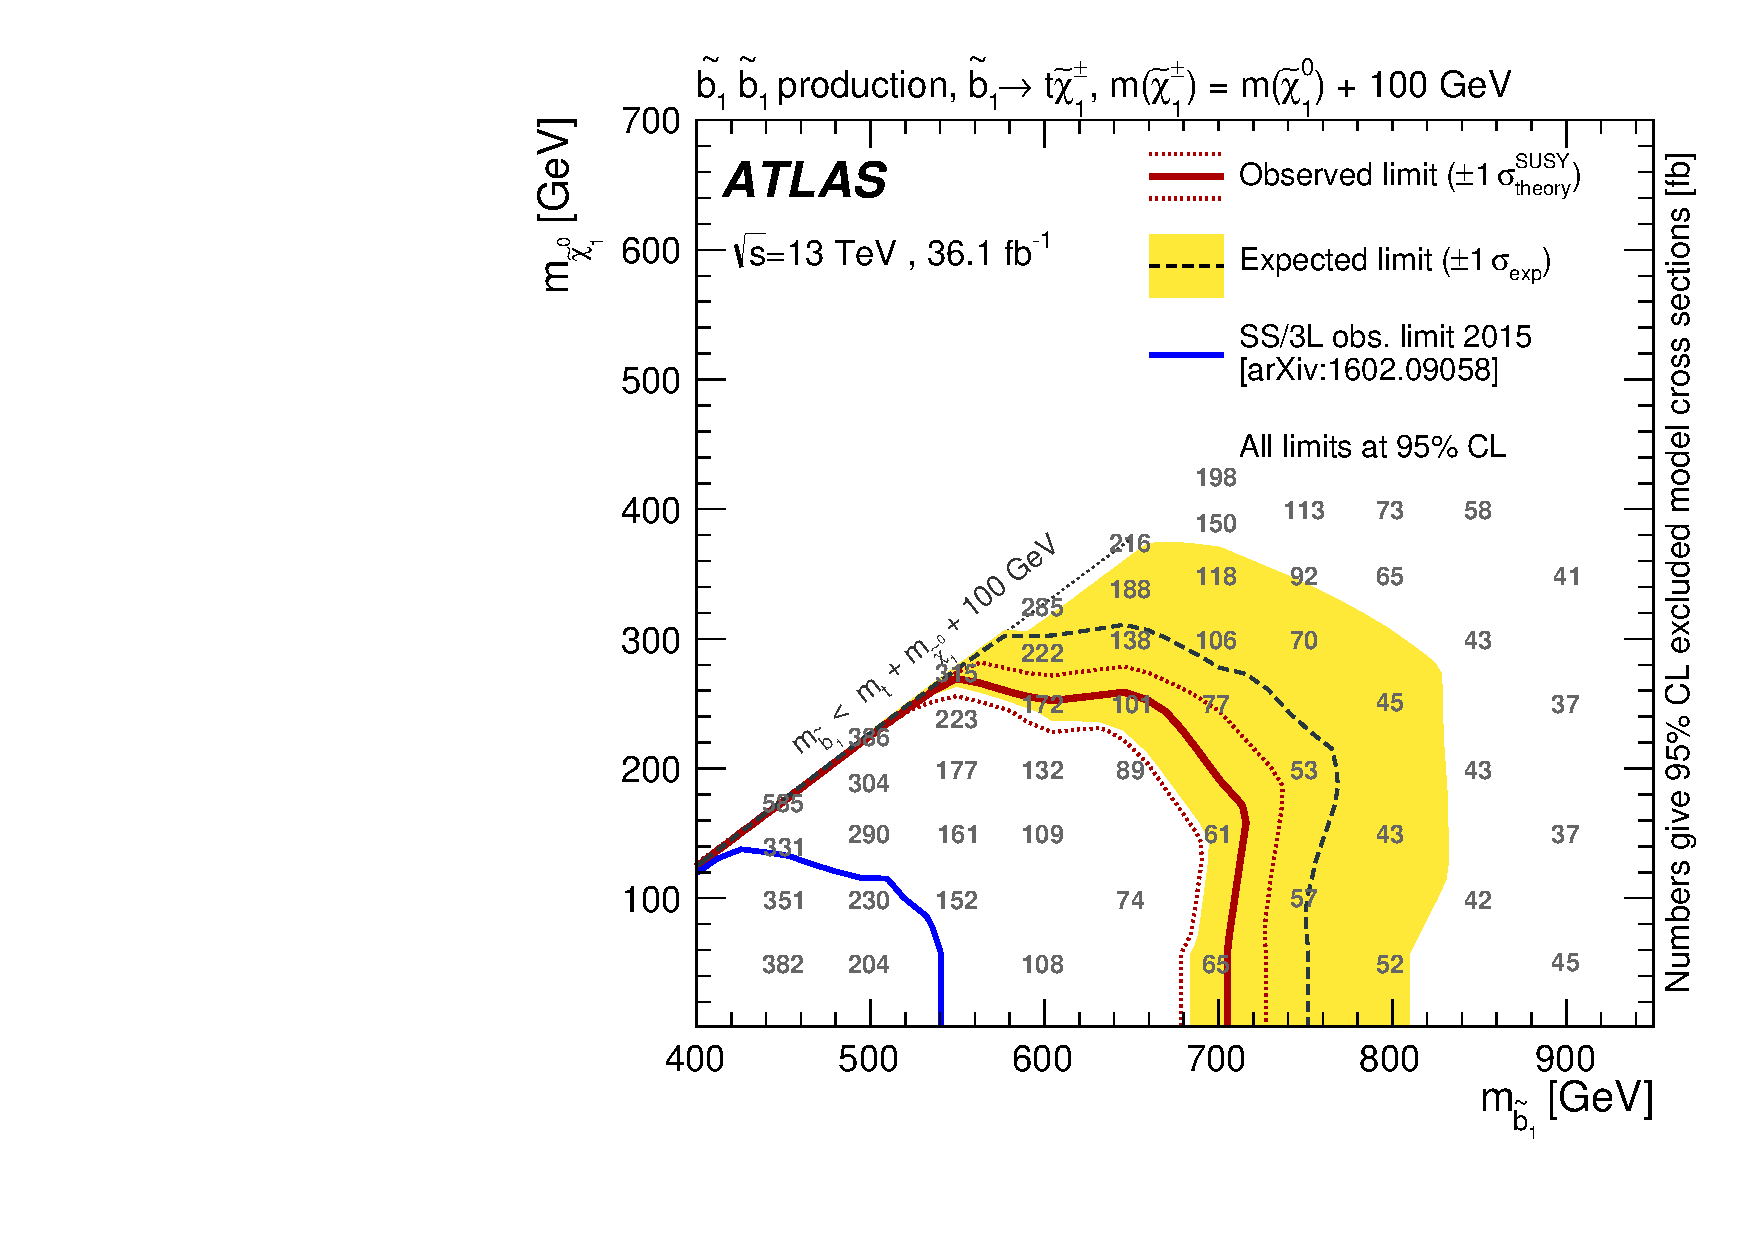
\includegraphics[width=\textwidth]{LIMITS/Btt_SRbest.pdf}\caption{Rpc2L1bS, Rpc2L1bH}\label{fig:limits_feynman_b1b1}\end{subfigure}
\begin{subfigure}[t]{0.38\textwidth}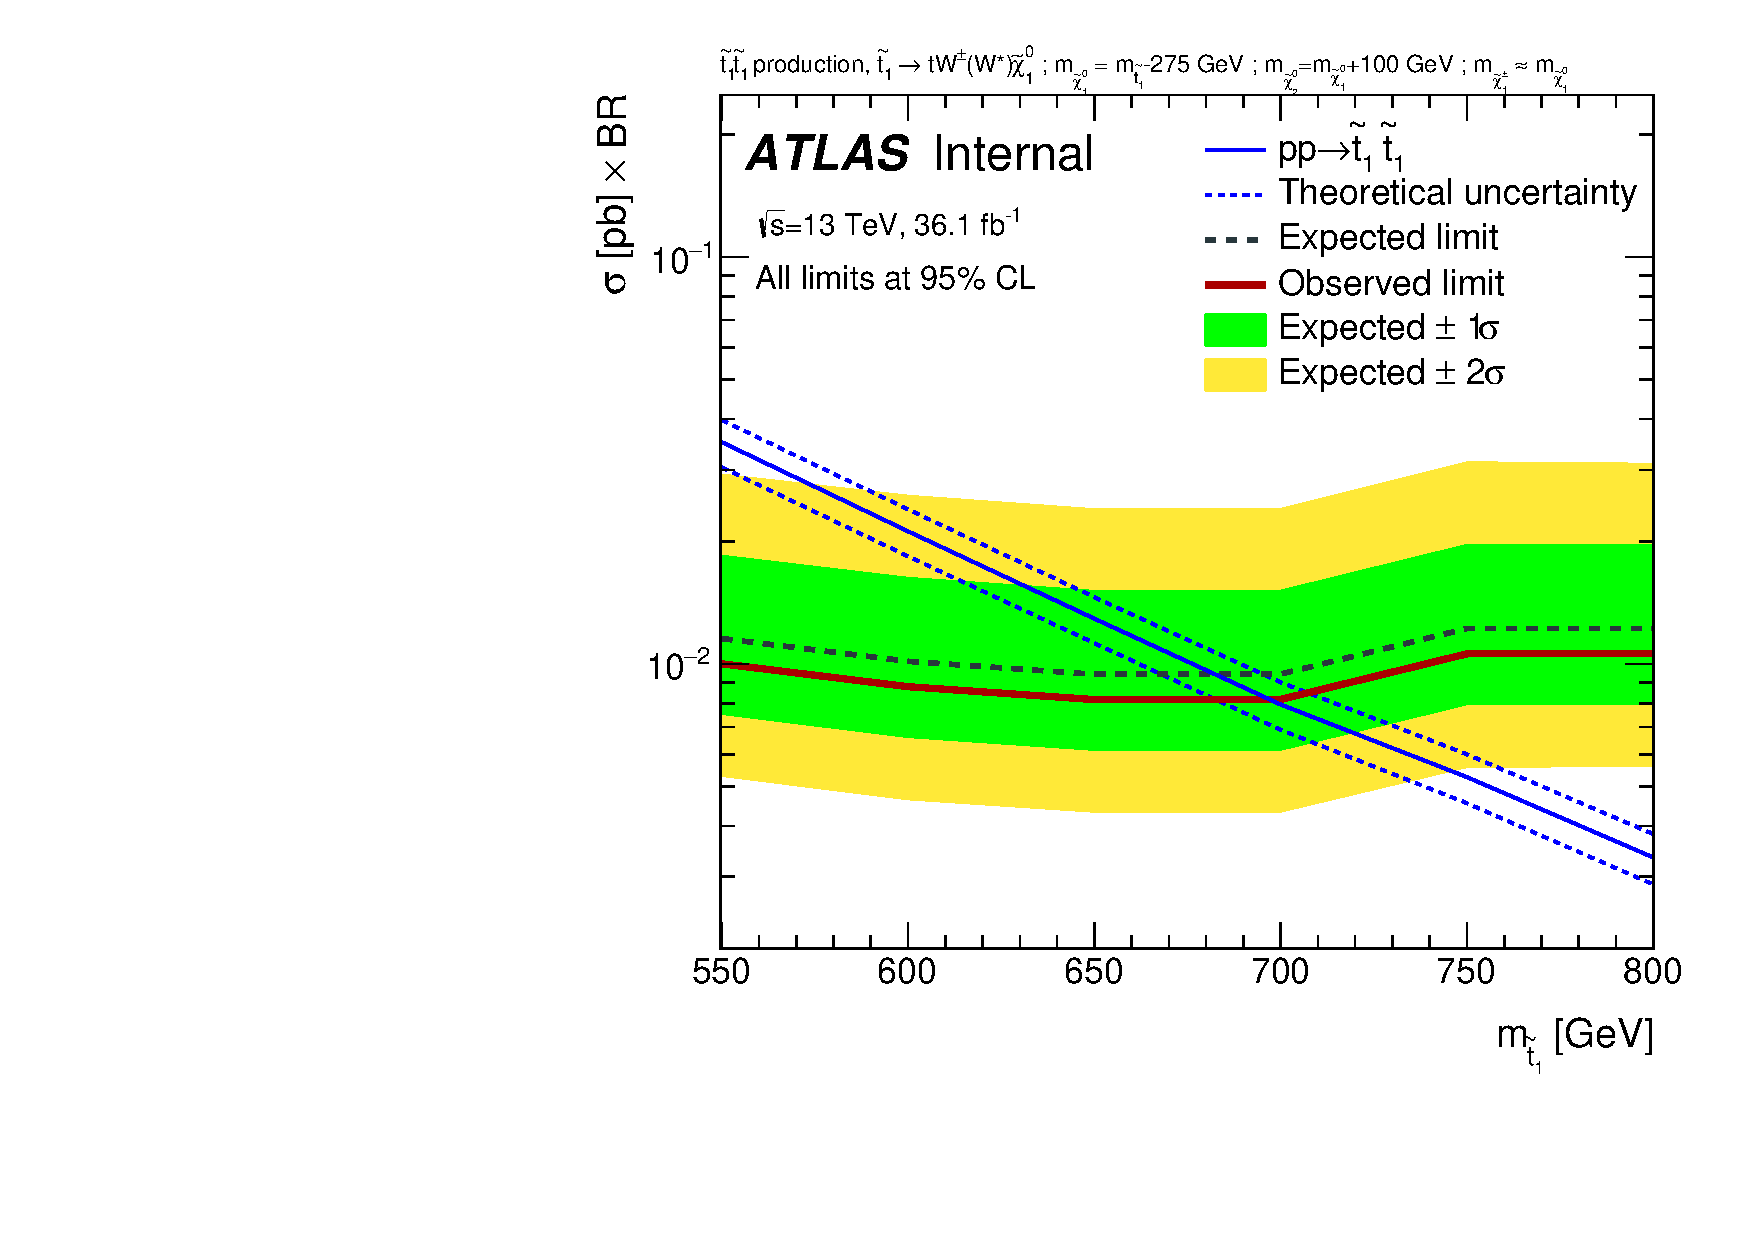
\includegraphics[width=\textwidth]{LIMITS/UL_TT2Step.pdf}\caption{Rpc3LSS1b}\label{fig:limits_feynman_t1t1}\end{subfigure}
\caption{Observed and expected exclusion limits on the $\tilde{g}$, \sbottomone, \stopone and \ninoone masses 
in the context of RPC SUSY scenarios with simplified mass spectra. The signal regions used to obtain the limits are specified in the subtitle of 
each scenario. All limits are computed at 95\% CL. The dotted lines around the observed
limit illustrate the change in the observed limit as the nominal signal cross-section is scaled up and down
by the theoretical uncertainty. The contours of the band around the expected 
limit are the $\pm$1$\sigma$ results ($\pm$2$\sigma$ is also considered in Figure~\ref{fig:limits_feynman_t1t1}), 
including all uncertainties except the theoretical ones in the signal cross-section. In Figures~\ref{fig:limits_feynman_gtt}--\ref{fig:limits_feynman_b1b1}, 
the grey diagonal line indicates the kinematic limit for the decays in each specified scenario and results are compared with the observed limits obtained 
by previous ATLAS searches~\cite{paperSS3L,Aad:2016jxj}.}
\label{fig:Results_Limits_RPC} 
\end{figure} 

\begin{figure}[b]
\centering
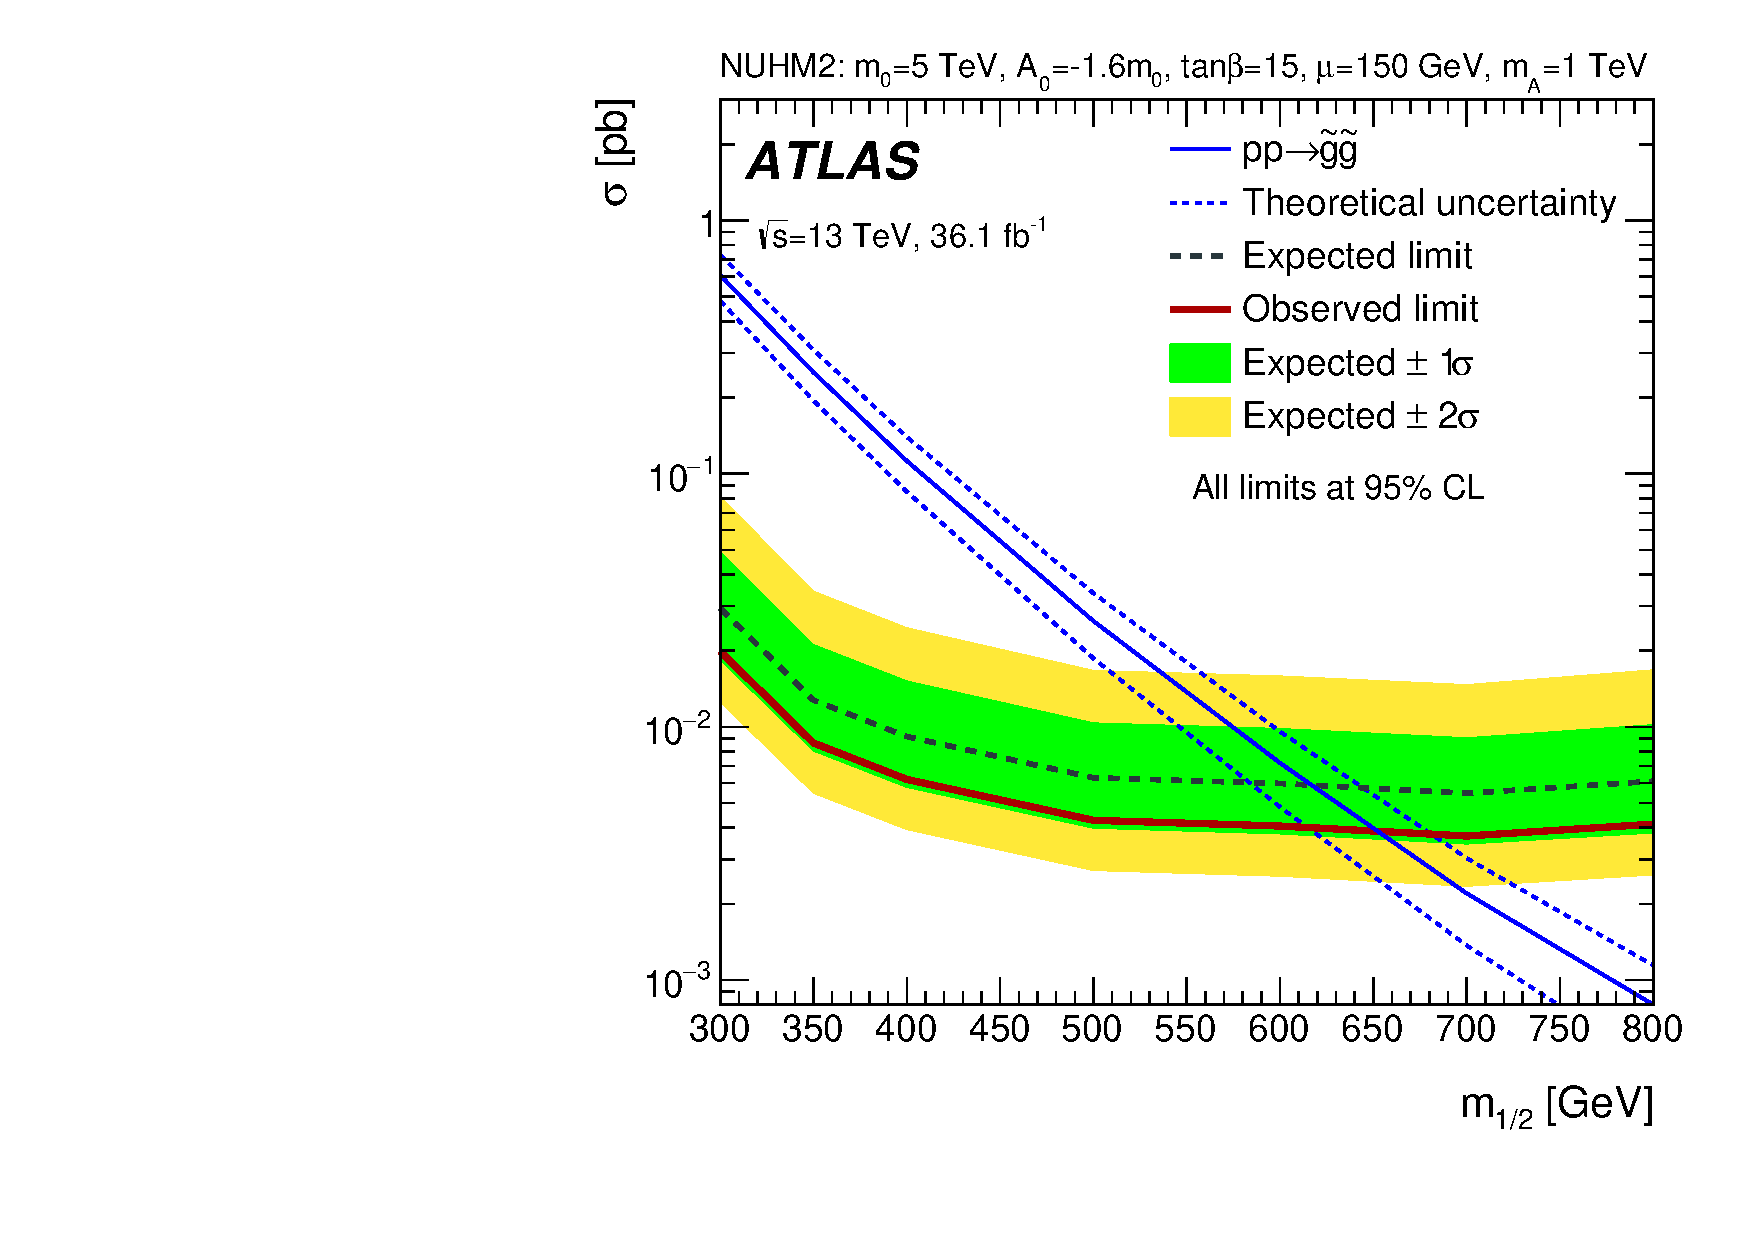
\includegraphics[width=0.70\textwidth]{LIMITS/UL_NUHM2}
\caption{Observed and expected exclusion limits as a function of $m_{1/2}$ in the NUHM2 model~\cite{Ellis:2002iu,Ellis:2002wv}.
The signal region Rpc2L2bH is used to obtain the limits. 
The contours of the green (yellow) band around the expected limit are the $\pm$1$\sigma$ ($\pm$2$\sigma$) results, including all uncertainties. The limits are computed at 95\% CL.}
\label{fig:Results_Limits_NUHM2} 
\end{figure} 

Exclusion limits at 95\% CL are also set on the masses of the superpartners involved in the SUSY benchmark scenarios considered. 
Apart from the NUHM2 model, simplified models are used, corresponding to a single production mode and with 100\% branching ratio to a specific decay chain, 
with the masses of the SUSY particles not involved in the process set to very high values. 
Figures~\ref{fig:Results_Limits_RPC} and \ref{fig:Results_Limits_NUHM2} show the exclusion limits in all 
the models considered in Figure~\ref{fig:feynman} and the NUHM2 model. The assumptions about the decay chain considered for the different SUSY particles are 
stated above each figure. For each region of the signal parameter space, the SR with the best expected sensitivity is chosen.

For the RPC models, the limits set are compared with the existing limits set by other ATLAS SUSY 
searches~\cite{paperSS3L,Aad:2016jxj}. For the models shown in Figure~\ref{fig:Results_Limits_RPC}, 
the mass limits on gluinos and bottom squarks are up to 400~GeV higher than the previous limits, reflecting the improvements 
in the signal region definitions as well as the increase in integrated luminosity. Gluinos with masses up to 1.75~TeV
are excluded in scenarios with a light $\ninoone$ in Figure~\ref{fig:limits_feynman_gtt}. This limit is extended to 1.87~TeV when 
$\ninotwo$ and slepton masses are in between the gluino and the $\ninoone$ masses (Figure~\ref{fig:limits_feynman_gg2sl}). More generally, gluino masses 
below 1.57~TeV and bottom squarks with masses below 700 GeV 
are excluded in models with a massless LSP. The ``compressed'' regions, where SUSY particle masses are close to each other, are also better covered 
and LSP masses up to 1200 and 250~GeV are excluded in the gluino and bottom squark pair-production models, respectively. Of particular
interest is the observed exclusion of models producing gluino pairs with an off-shell top quark in the decay (Figure~\ref{fig:feynman_gttOffshell}), 
see Figure~\ref{fig:limits_feynman_gtt}. In this case, models are excluded for mass differences between the gluino and neutralino of 205 GeV (only ~35 GeV
larger than the minimum mass difference for decays into two on-shell $W$ bosons and two $b$-quarks) for a gluino mass below 0.9
TeV. The Rpc3LSS1b SR allows the exclusion of top squarks with masses below 700~GeV when the top squark decays to a top quark and a cascade of electroweakinos 
$\ninotwo \to \chinoonepm W^{\mp} \to W^{*} W^{\mp} \ninoone$ (see Figure~\ref{fig:limits_feynman_t1t1} for the conditions 
on the sparticle masses).


Finally, in the NUHM2 model with low fine-tuning, values of the parameter $m_{1/2}$ below 615 GeV are excluded, 
corresponding to gluino masses below 1500 GeV (Figure~\ref{fig:Results_Limits_NUHM2}).
